\documentclass[a4paper,10pt]{article}
% Allow the usage of UTF-8 characters

\usepackage[left=10mm, top=20mm, right=18mm, bottom=15mm, footskip=10mm]{geometry}
\usepackage{geometry}


\usepackage[utf8]{inputenc}
\usepackage[T2A] {fontenc}
\usepackage[russian]{babel}
% Allow the usage of graphics (.png, .jpg)
\usepackage{graphicx}

\usepackage{pifont}
\usepackage{amsmath}

\title{1.4.8. Измерение модуля Юнга путем акустического резонанаса}
\author{Комиссаров Данил Б01-307}
\date{Ноябрь 2023}

\begin{document}
	
	\maketitle
	
	\section{Основные формулы}
	\begin{equation}
		f_1 = u / 2L
		\label{estimated f1}
	\end{equation}
	
	\begin{equation}
		x_\text{ср} = \frac{1}{n}\sum^n_{i=1}{x_i}
		\label{x mid}
	\end{equation}
	
	\begin{equation}
		\sigma_\text{отд} = \sqrt{\frac{1}{n - 1}\sum^n_{i=1}{(x_i = x_\text{ср})^2}}
		\label{exp fault}
	\end{equation}
	
	\begin{equation}
		\varepsilon_k = \frac{\sigma_k}{k}
		\label{rel fault}
	\end{equation}
	
	\begin{equation}
		\rho = \frac{4m}{\pi d^2 l}
		\label{density}
	\end{equation}
	
	\begin{equation}
		u = 2L\frac{f_n}{n}
		\label{sound spped}
	\end{equation}
	
	\begin{equation}
		E = c_\text{ст}^2 \rho
		\label{Ung}
	\end{equation}
	\begin{equation}
		\Delta E = E \sqrt{4(\frac{\delta c_\text{ст}}{c_\text{ст}})^2 + (\frac{\delta\rho}{\rho})^2}
		\label{Ung acc}
	\end{equation}
	
	\section{Обработка результатов}
	\subsection{Медь}
	Предварительно оценим частоту первого резонанаса по формуле (\ref{estimated f1}).
	\[f_1 = 3.06 \text{ кГц}\] 
	Путем перестройки звукогого гененратора был найден первый резонанс $f_1 = 3.151$ кГц. На экране наблюдается эллипс.
	\begin{center}
		\begin{tabular}{|c||c|c|c|c|}
			\hline
			Измерения (кГц) & 1 & 2 & 3 & 4 \\
			\hline
			& 3.151 & 3.152 & 3.151 & 3.150 \\
			\hline
		\end{tabular}
	\end{center}
	По формулам (\ref{x mid}) и (\ref{exp fault}) находим, что экспериментальная погрешность равна $\sigma = 8 * 10^{-4} \text{кГц}$. Или же относительная погрешность по (\ref{rel fault}): $\varepsilon_x = 2 * 10^{-4}$.
	Найдем частоты, на кратных гармониках: 
	\begin{center}
		\begin{tabular}{|c||c|c|c|c|c|c|c|c|c|c|c|c|c|}
			\hline
			Измерения (кГц) & 1 & 2 & 3 & 4 & 5 & 6 & 7 & 8 & 9 & 10\\
			\hline
			& 3.151 & 6.326 & 9.482 & 12.647 & 15.801 & 18.970 & 22.106 & 25.251 & 28.386 & 31.552 \\
			\hline
		\end{tabular}
	\end{center}
	Найдем плотность медного стержня $d = (1.185 \pm 0.001) \text{ см}$, $l = (3.05 \pm 0.01) \text{ см}$, $m = (29.437 \pm 0.001) \text{ г}$ по (\ref{density}).
	
	$\rho = (8755 \pm 31)$ кг/м$^3$.
	
	Определим среднеее значение диаметра медного стержня:
	\begin{center}
		\begin{tabular}{|c||c|c|c|c|}
			\hline
			Измерения (см) & 1 & 2 & 3 & 4 \\
			\hline
			& 1.20 & 1.20 & 1.19 & 1.21 \\
			\hline
		\end{tabular}
	\end{center}
	$d_\text{ср} = 1.2$ см.
	
	$\frac{d / 2}{l} = 9.9 * 10^{-3} << 1$ - стержень тонкий.
	
	Повторим опыты и для других стержней.
	\subsection{Дюраль}
	Частоты кратных гармоник: 
	\begin{center}
		\begin{tabular}{|c||c|c|c|c|c|c|c|c|c|c|}
			\hline
			Измерения (кГц) & 1 & 2 & 3 & 4 & 5 & 6 & 7 \\
			\hline
			& 4.257 & 8.537 & 12.775 & 17.038 & 21.289 & 25.559 & 29.762\\
			\hline
		\end{tabular}
	\end{center}
	
	$d = 1.173 \text{ см}$, $l = 4.14 \text{ см}$, $m = 12.443 \text{ г}$
	
	Плотность стержня (\ref{density}): $\rho = 2782$ кг/м$^3$.
	
	$d_\text{ср} = 1.17$ см.
	
	$\frac{d / 2}{l} = 9.6 * 10^{-3} << 1$ - стержень тонкий.
	\subsection{Сталь}
	Частоты кратных гармоник: 
	\begin{center}
		\begin{tabular}{|c||c|c|c|c|c|c|c|c|c|}
			\hline
			Измерения (кГц) & 1 & 2 & 3 & 4 & 5 & 6 \\
			\hline
			& 4.123 & 8.249 & 12.374 & 16.505 & 20.619 & 24.780\\
			\hline
		\end{tabular}
	\end{center}
	
	$d = 1.950 \text{ см}$, $l = 2.95 \text{ см}$, $m = 26.017 \text{ г}$
	
	Плотность стержня (\ref{density}): $\rho = 7673$ кг/м$^3$.
	
	$d_\text{ср} = 1.21$ см.
	
	$\frac{d / 2}{l} = 10^{-4} << 1$ - стержень тонкий.
	
	\subsection{Первая гамоника для дюрали}
	Модуляция на частоте $f = 1.579$ кГц.
	При этой частоте стержень входит в резонанс. Ось X показывает колебания самого генератора, ось Y показывает колебания с датчика. Стержень имеет собственную частоту $f = 4.257$ кГц - такая же частота сигналов с датчика, а генератор имеет частоту $f / 2$. Пока X Совершает отдно колебание, Y совершает 2 колебания, отсюда и такая фигура.
	
	\begin{center}
		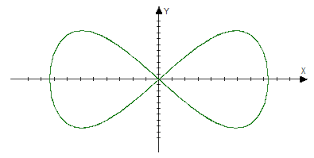
\includegraphics[width=0.5\textwidth]{лисссажу}
		\label{лисссажу}
	\end{center}
	
	\subsection{Добротность медного стержня}
	Напряжение при первом резонансе: $U = 13.5$ В.
	
	$\frac{U}{\sqrt{2}} = 9.5$ В.
	
	Частоты при таком напряжении: $\nu = 3.156 \text{ кГц}$, $\nu = 3.146 \text{ кГц}$
	
	$\Delta f = 10$ Гц.
	$Q = \frac{f}{\Delta f} = 315.1.$
	\subsection{График частоты}
	График зависимости частоты от номера гармоники
	\begin{center}
		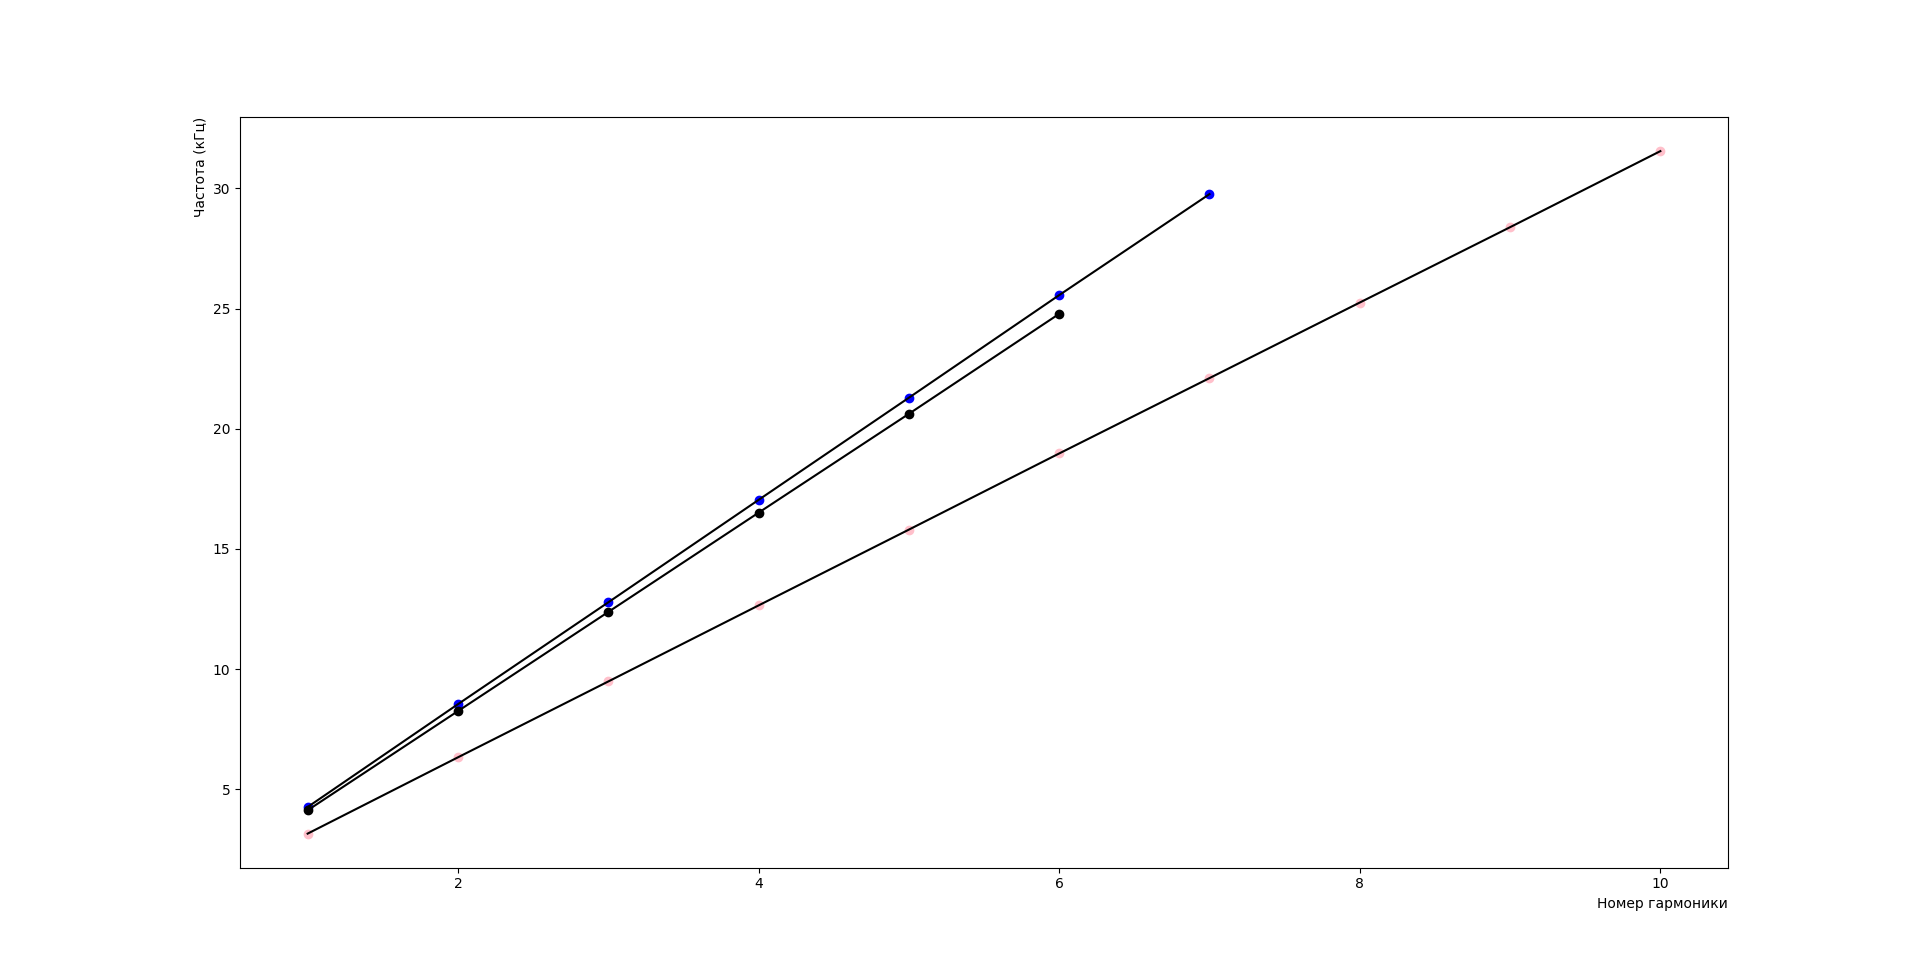
\includegraphics[width=1.2\textwidth]{Частоты гармоник.png}
		\label{Частоты гармоник}
	\end{center}
	*верхняя прямая соответствует дюрали, средняя - стали, нижняя - меди.
	
	Ниже график аппроксимированной прямой для меди с погрешностями (прямые погрешностей практически совпадает с апроксисмированной прямой).
	\begin{center}
		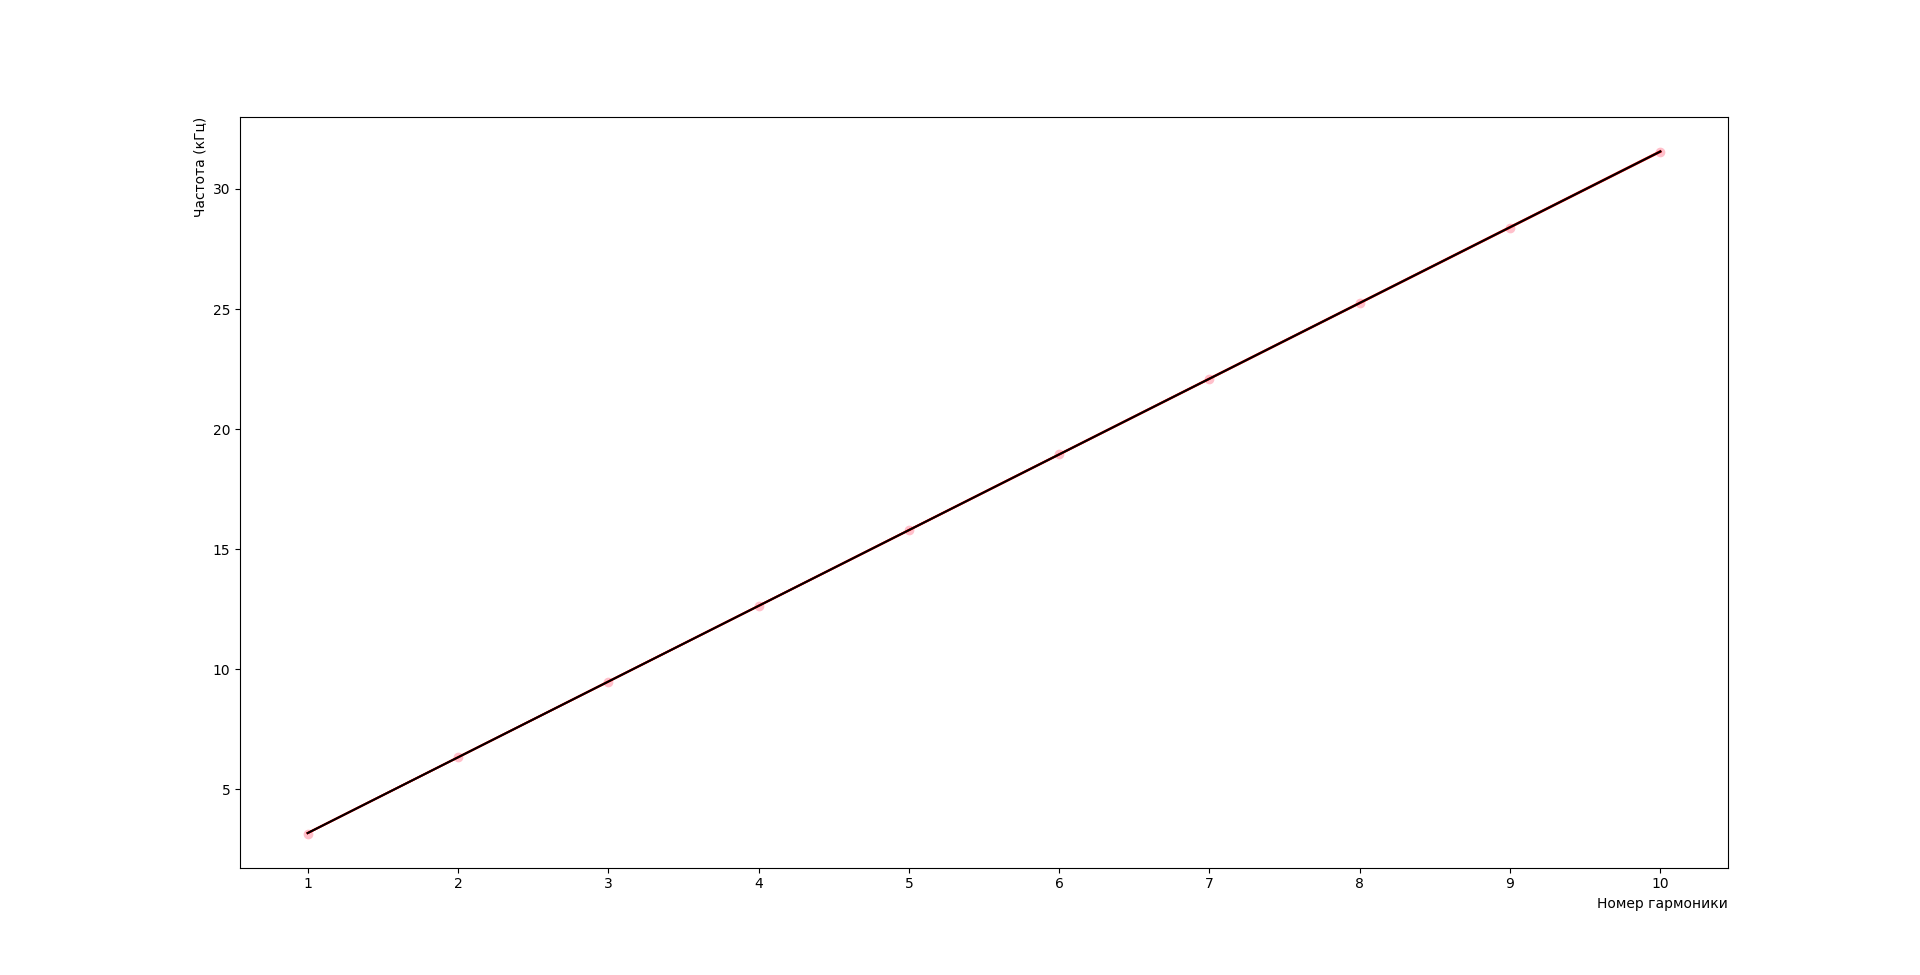
\includegraphics[width=1.2\textwidth]{медь апрокс.png}
		\label{медь апрокс}
	\end{center}
	
	\subsection{Скорость звука}
	По (\ref{sound spped}) скорость звука равна:\\
	Для меди: $u = (3808.8 \pm 8.1)\text{ м/с}^2$ (0.21\%) \\
	Для дюрали: $u = (5152.2 \pm 6.1)\text{ м/с}^2$ (0.11\%) \\
	Для стали: $u = (4991.7 \pm 3.1)\text{ м/с}^2$ (0.06\%) \\
	(погрешность измерения длины стержня пренебрежительно мала, по сравнению с погрешностью $\frac{f_n}{n}$)
	
	\subsection{Определение модуля Юнга}
	Воспользуемся формулами (\ref{Ung}) и (\ref{Ung acc}), тогда:\\
	Для меди: $E = (127.0 \pm 0.7)\text{ ГПа}$ (0.55\%) \\
	Для дюрали: $E = (73.8 \pm 0.3)\text{ ГПа}$ (0.42\%) \\
	Для стали: $E = (191.2 \pm 0.7)\text{ ГПа}$ (0.38\%)
	\section{Вывод}
	Измерение модуля Юнга путем акустического резонанса является достаточно надежным методом.
\end{document}
